\begin{figure}[!htb]
  \centering
  \begin{subfigure}{0.23\textwidth}
    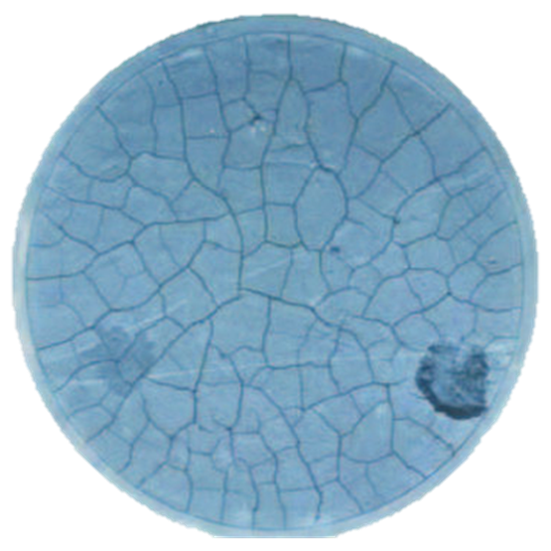
\includegraphics[width=\textwidth,scale=0.5]{Chapter4/figures/3D/4mm_exp.png}
    \caption{}
  \end{subfigure}
  \hspace{0.05\textwidth}
  \begin{subfigure}{0.23\textwidth}
    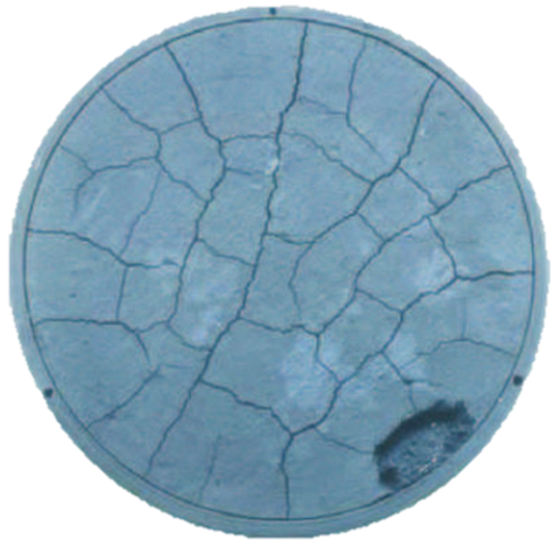
\includegraphics[width=\textwidth,scale=0.5]{Chapter4/figures/3D/8mm_exp.png}
    \caption{}
  \end{subfigure}
  \hspace{0.05\textwidth}
  \begin{subfigure}{0.23\textwidth}
    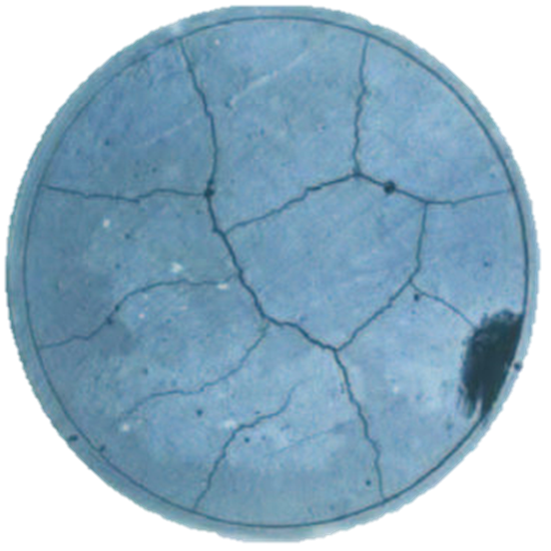
\includegraphics[width=\textwidth,scale=0.5]{Chapter4/figures/3D/16mm_exp.png}
    \caption{}
  \end{subfigure}
  
  \begin{subfigure}{0.23\textwidth}
    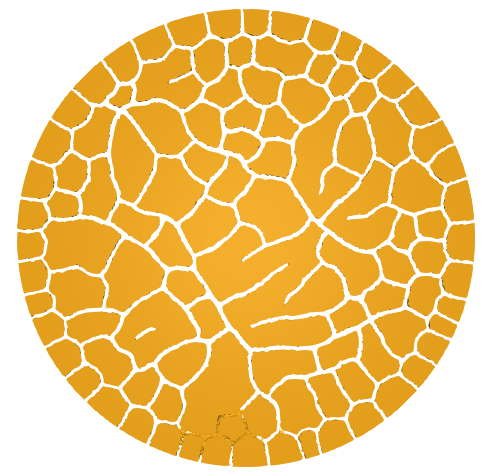
\includegraphics[width=\textwidth,scale=0.5]{Chapter4/figures/3D/4mm_top.png}
    \caption{}
  \end{subfigure}
  \hspace{0.05\textwidth}
  \begin{subfigure}{0.23\textwidth}
    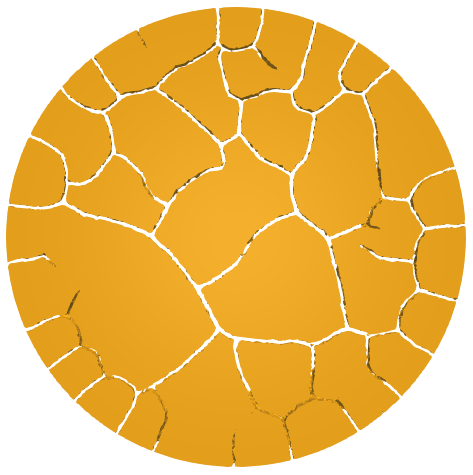
\includegraphics[width=\textwidth,scale=0.5]{Chapter4/figures/3D/8mm_top.png}
    \caption{}
  \end{subfigure}
  \hspace{0.05\textwidth}
  \begin{subfigure}{0.23\textwidth}
    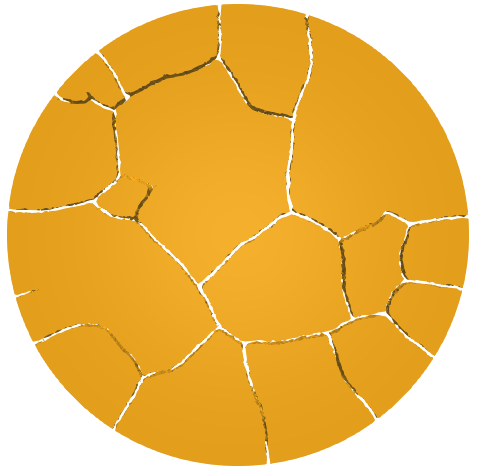
\includegraphics[width=\textwidth,scale=0.5]{Chapter4/figures/3D/16mm_top.png}
    \caption{}
  \end{subfigure}
  
  \begin{subfigure}{0.23\textwidth}
    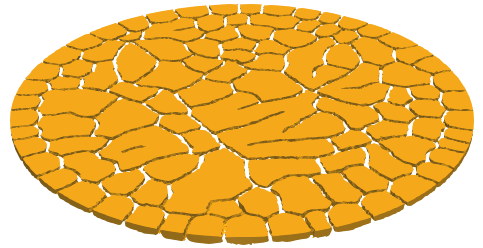
\includegraphics[width=\textwidth,scale=0.5]{Chapter4/figures/3D/4mm_3D.png}
    \caption{}
  \end{subfigure}
  \hspace{0.05\textwidth}
  \begin{subfigure}{0.23\textwidth}
    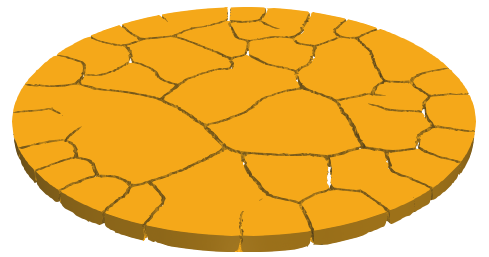
\includegraphics[width=\textwidth,scale=0.5]{Chapter4/figures/3D/8mm_3D.png}
    \caption{}
  \end{subfigure}
  \hspace{0.05\textwidth}
  \begin{subfigure}{0.23\textwidth}
    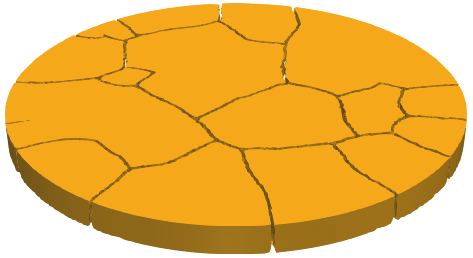
\includegraphics[width=\textwidth,scale=0.5]{Chapter4/figures/3D/16mm_3D.png}
    \caption{}
  \end{subfigure}
  \caption[Qualitative comparison between the experiments and the simulations with different thickness.]{Qualitative comparison between the experiments and the simulations: (a-c) Photographs (modified from \cite{Rodriguez2006}) of  cracks in mining waste due to desiccation at steady state for three test specimens with thickness (a) \SI{4}{\milli\meter}, (b) \SI{8}{\milli\meter}, and (c) \SI{16}{\milli\meter}.  (d-f) Top view and (g-i) panoramic view of corresponding numerical simulation results with different film thickness.  Volumes of material with $d \geqslant 0.75$ were removed to improve the visualization of the crack geometry. }
  \label{fig: Chapter4/3D/3D}
\end{figure}
